
% This LaTeX was auto-generated from an M-file by MATLAB.
% To make changes, update the M-file and republish this document.

\documentclass{article}
\usepackage{graphicx}
\usepackage{color}

\sloppy
\definecolor{lightgray}{gray}{0.5}
\setlength{\parindent}{10pt}
\usepackage[margin=1in]{geometry}

\begin{document}

\title{Dynamical Adaptation in ORNs}
\author{Srinivas Gorur-Shandilya}
\maketitle

    
    
\subsection*{Contents}

\begin{itemize}
\setlength{\itemsep}{-1ex}
   \item Rough Overview of Data
   \item Trial to Trial variability
   \item Data Statistics and Linear Fit
   \item Gain Analysis: Comparison to Linear Model
   \item Fitting a DA Model
   \item Gain Analysis: Comparison to DA Model
\end{itemize}
\begin{par}
How do ORNs respond to non-Gaussian inputs? Real odor stimuli are characterised by long tails and non-gaussian statisitcs, with large whiffs of odor that occur in periods of relatively low signal. Such a stimulus has been generated here, and the responses of ORNs to these signals is analysed in this figure.
\end{par} \vspace{1em}


\subsection*{Rough Overview of Data}

\begin{par}
The following figure shows what the stimulus and the neuron's response looks like.
\end{par} \vspace{1em}

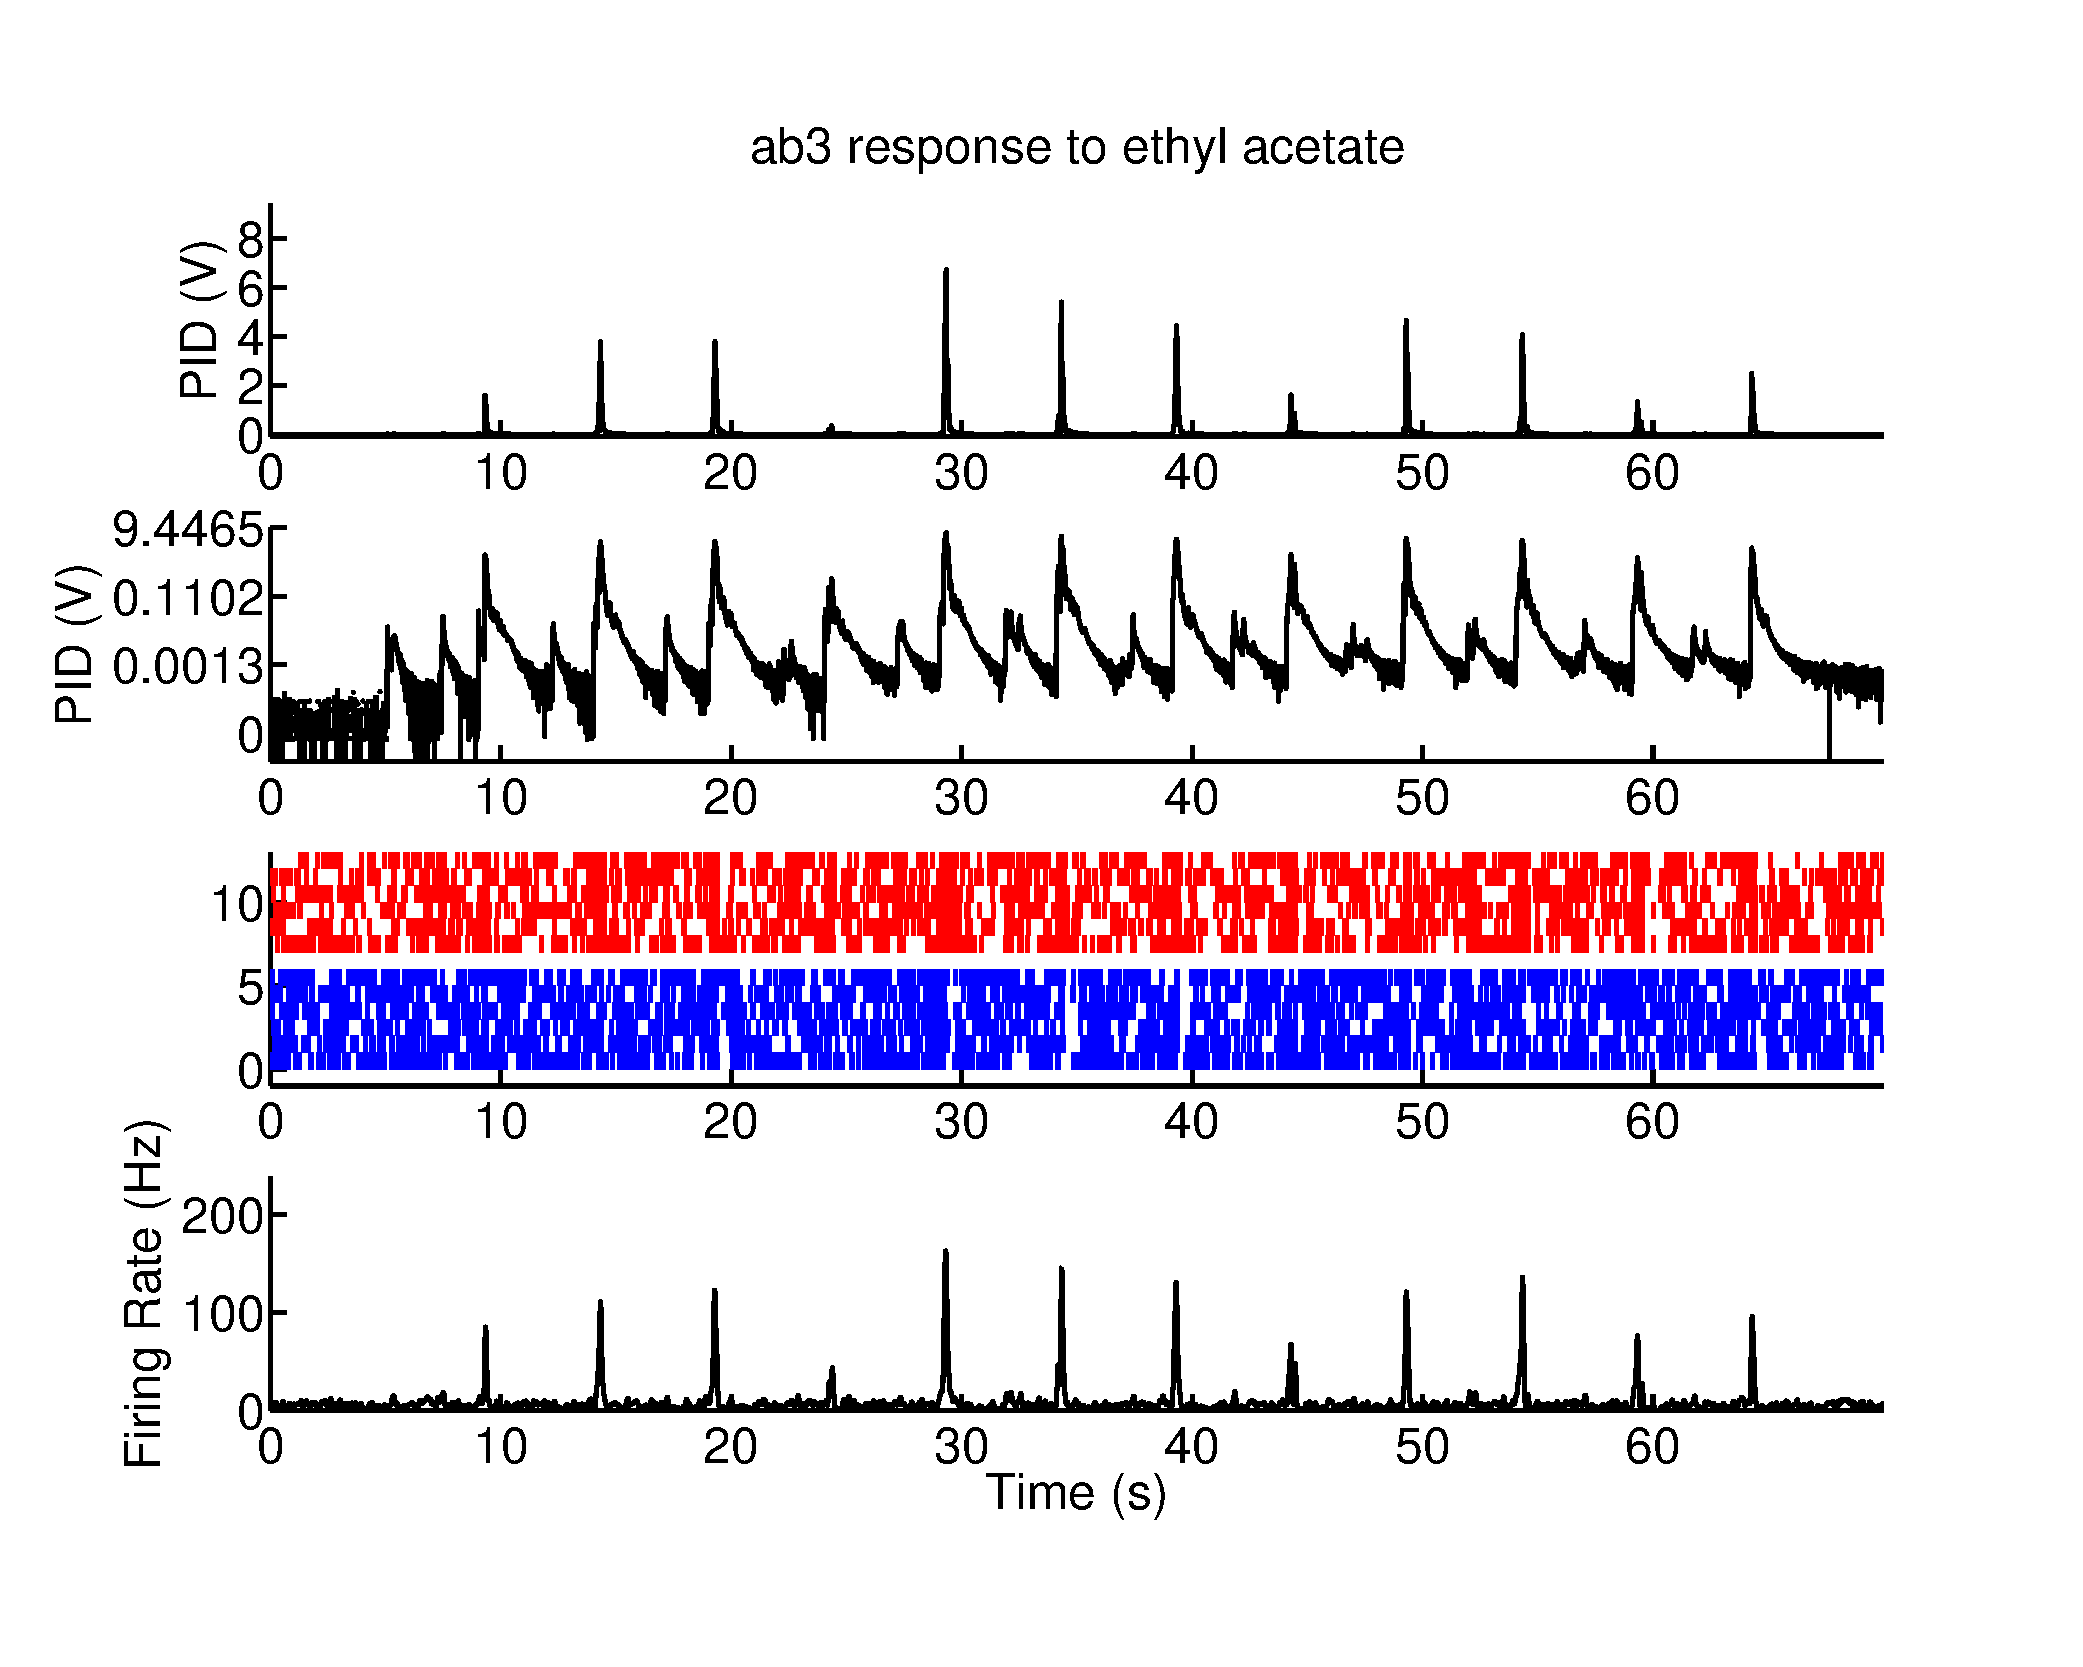
\includegraphics [width=\textwidth]{Mahmut_Data_Analysis_01.pdf}


\subsection*{Trial to Trial variability}

\begin{par}
How variable is the response and the stimulus from trial to trial? The following figure shows individual traces of the stimulus and the neuron's response for each trial.
\end{par} \vspace{1em}

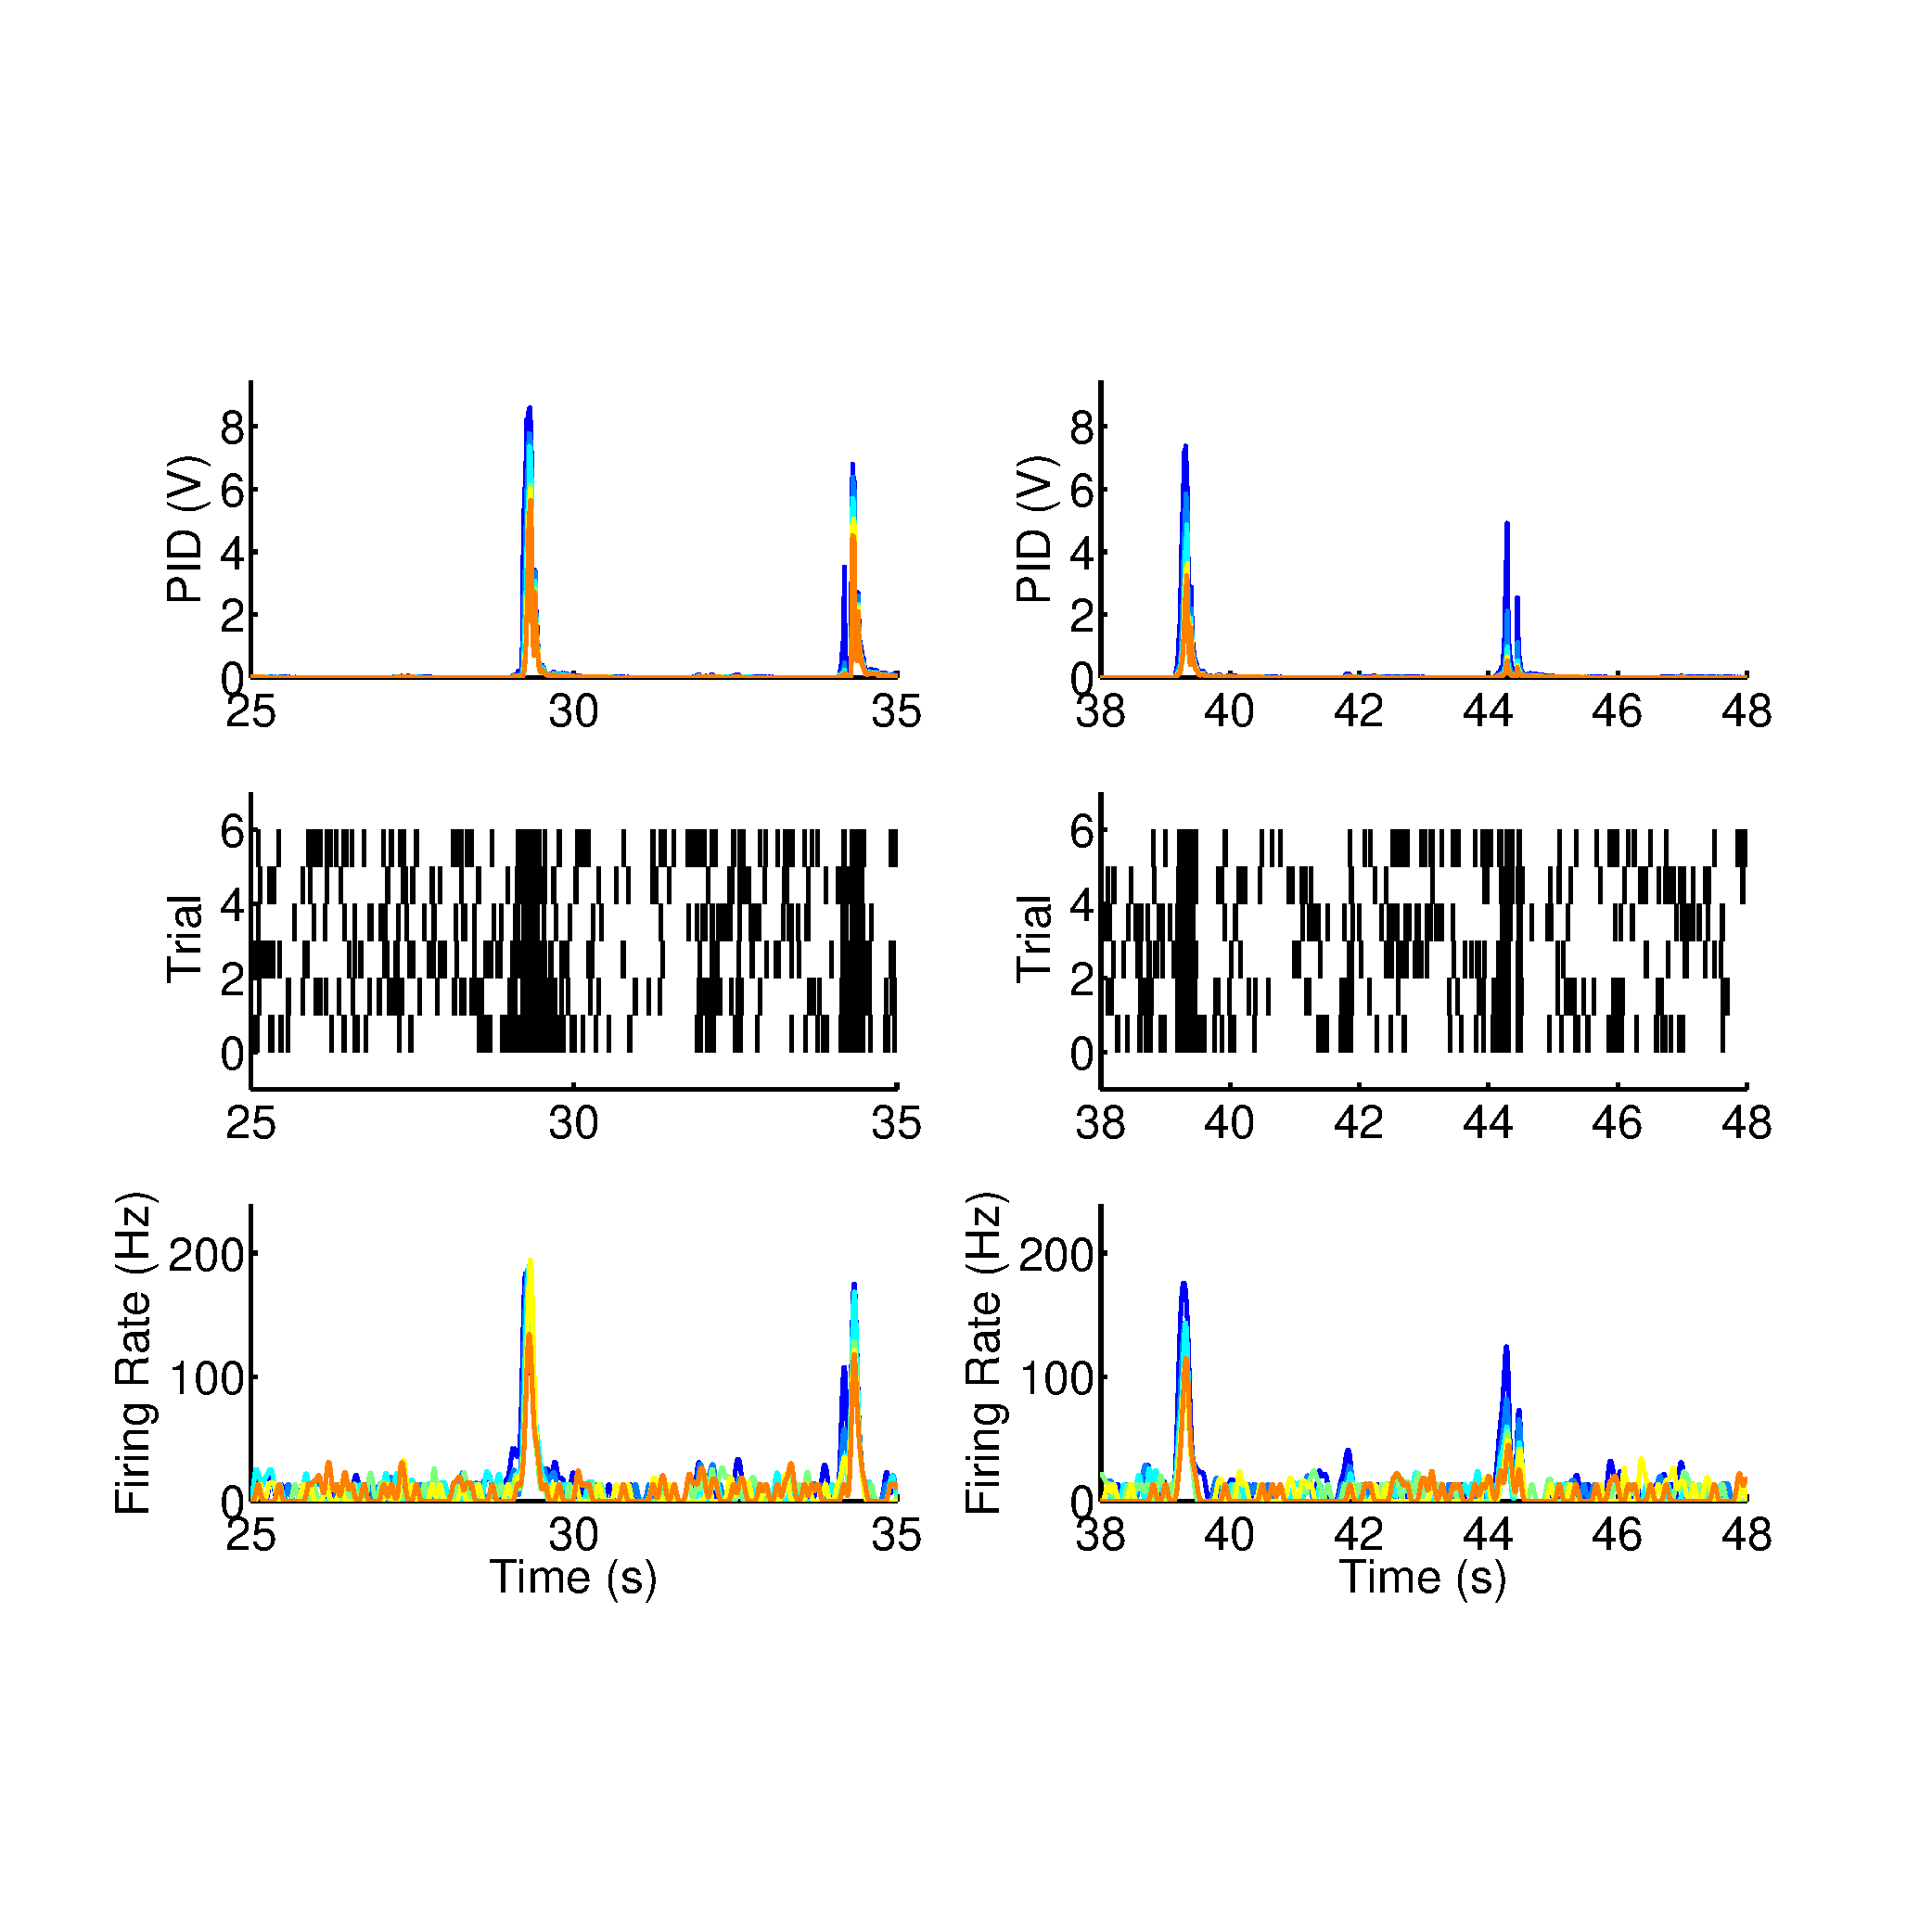
\includegraphics [width=\textwidth]{Mahmut_Data_Analysis_02.pdf}
\begin{par}
It looks like the amplitude of the signal is dropping every trial, but that the response amplitude isn't changing much (see the whiff at $t=39s$).
\end{par} \vspace{1em}
\begin{par}
To quantify this, let's attempt to find all the times when the stimulus is high, i.e., ten standard deviations above the baseline. This threshold ensures that we pick up all the whiffs, but ignore the blanks in between, as shown in the figure below.
\end{par} \vspace{1em}

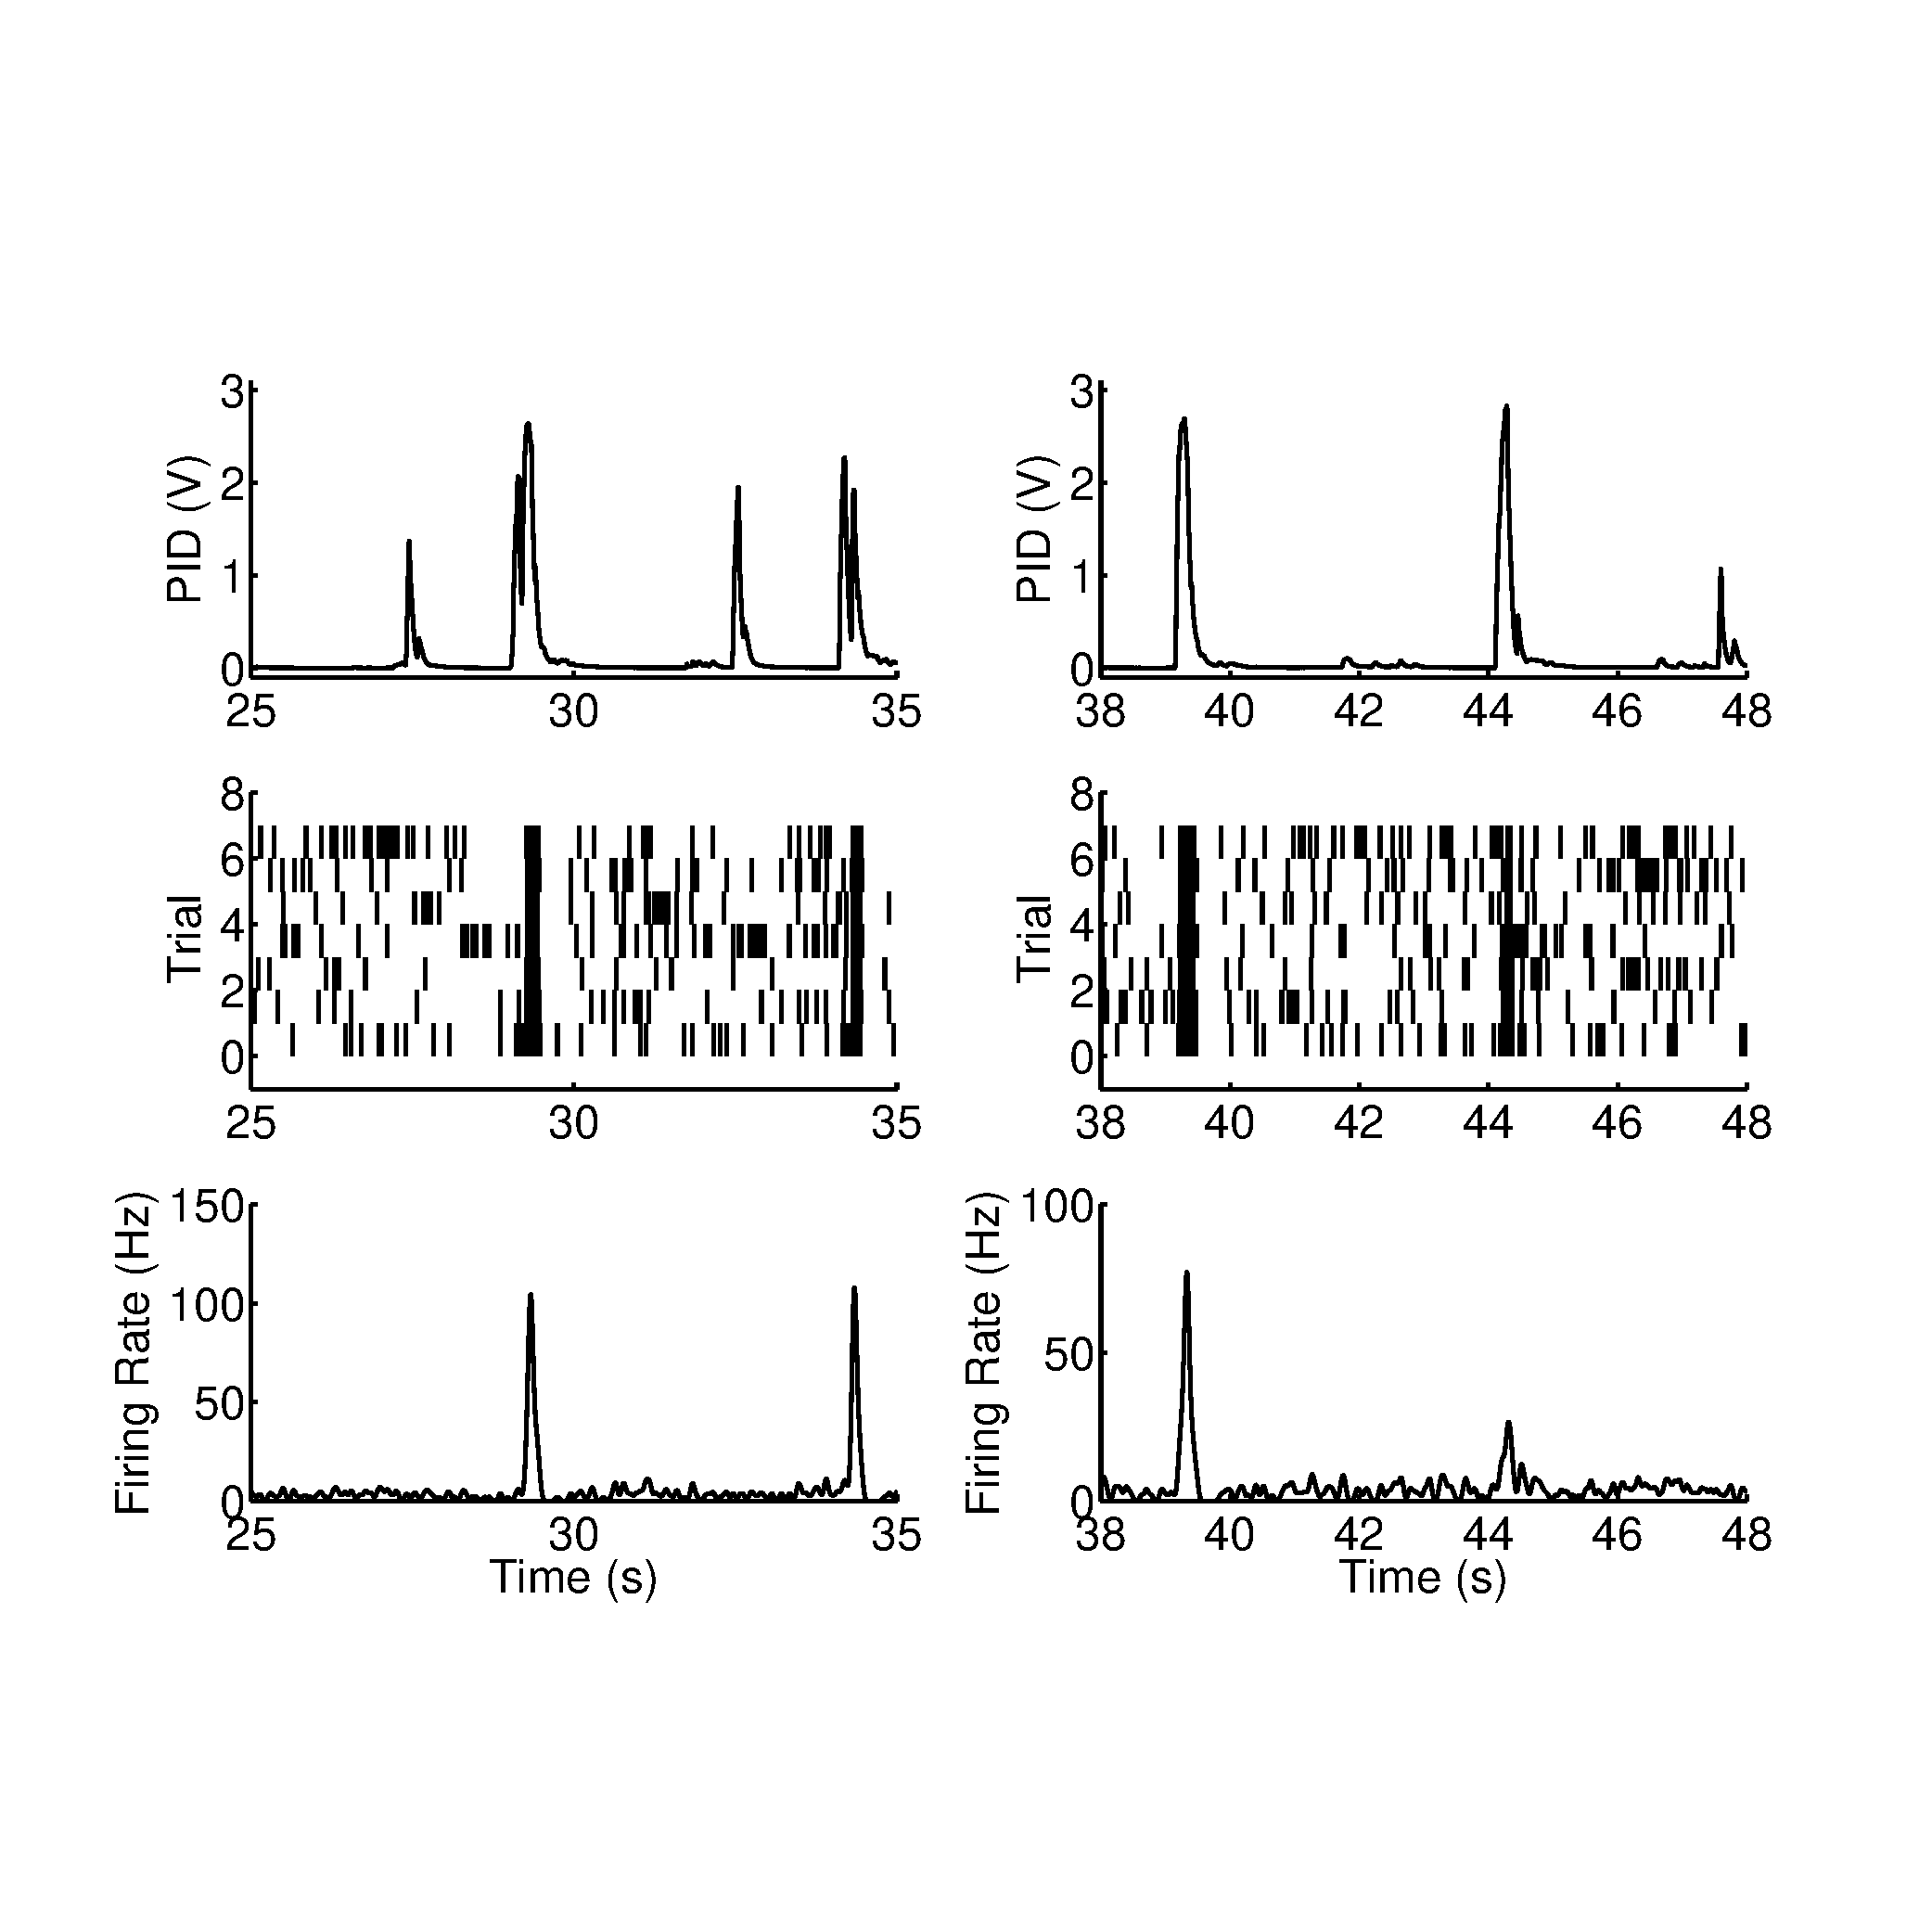
\includegraphics [width=\textwidth]{Mahmut_Data_Analysis_03.pdf}
\begin{par}
Now we break up the trace so that we can perform a whiff-by-whiff analysis of the stimulus and the response, for each trial. The following figure shows how the whiff amplitude and response amplitude drop as a function of trial number.
\end{par} \vspace{1em}

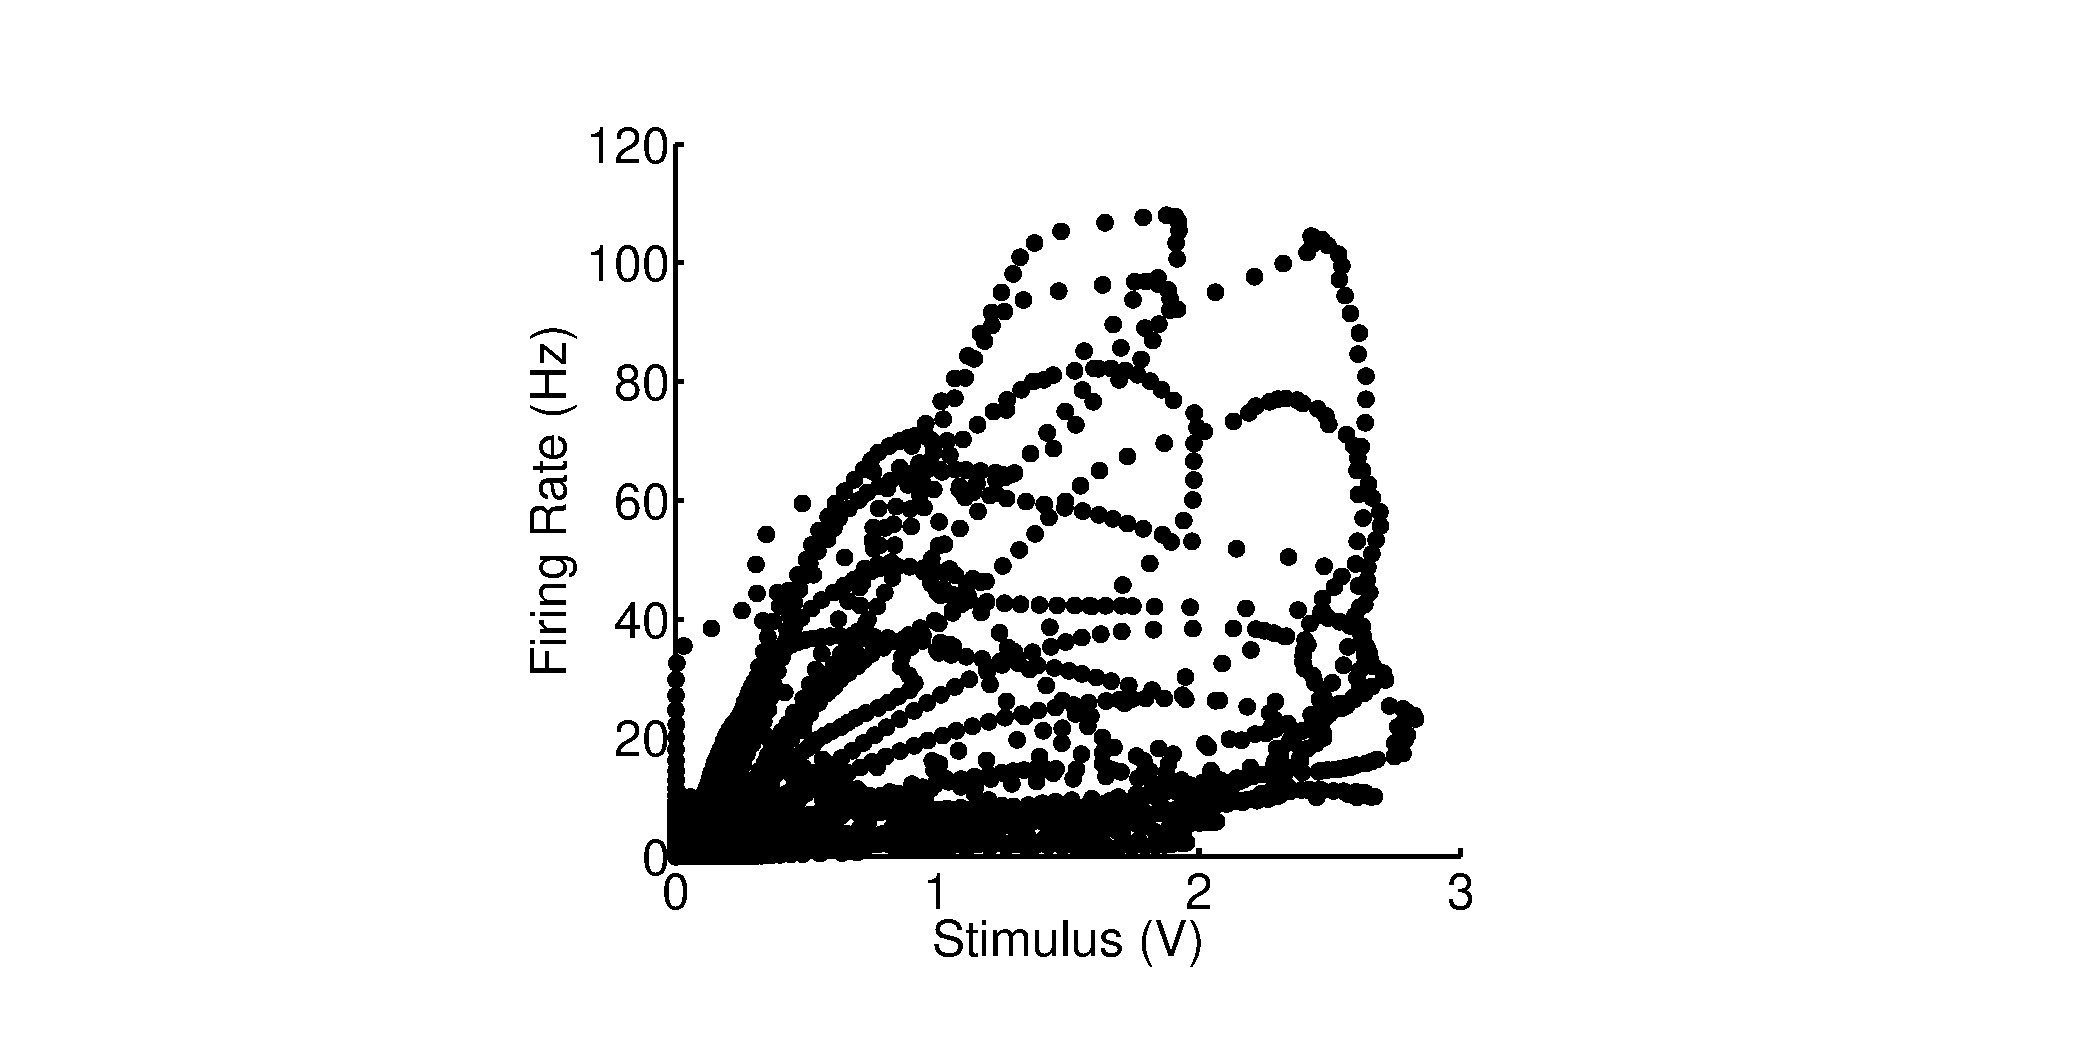
\includegraphics [width=\textwidth]{Mahmut_Data_Analysis_04.pdf}
\begin{par}
This captures what we see before, that even though the stimulus drops precipitously from trial to trial, the neuron response seems relatively unchanged.
\end{par} \vspace{1em}


\subsection*{Data Statistics and Linear Fit}

\begin{par}
The following figure describes the statistics of the stimulus and the response. Left panel: Histograms of stimulus and response. Middle panel: Autocorrelation functions of the stimulus and the response. Right: Linear filter extracted from this dataset.
\end{par} \vspace{1em}

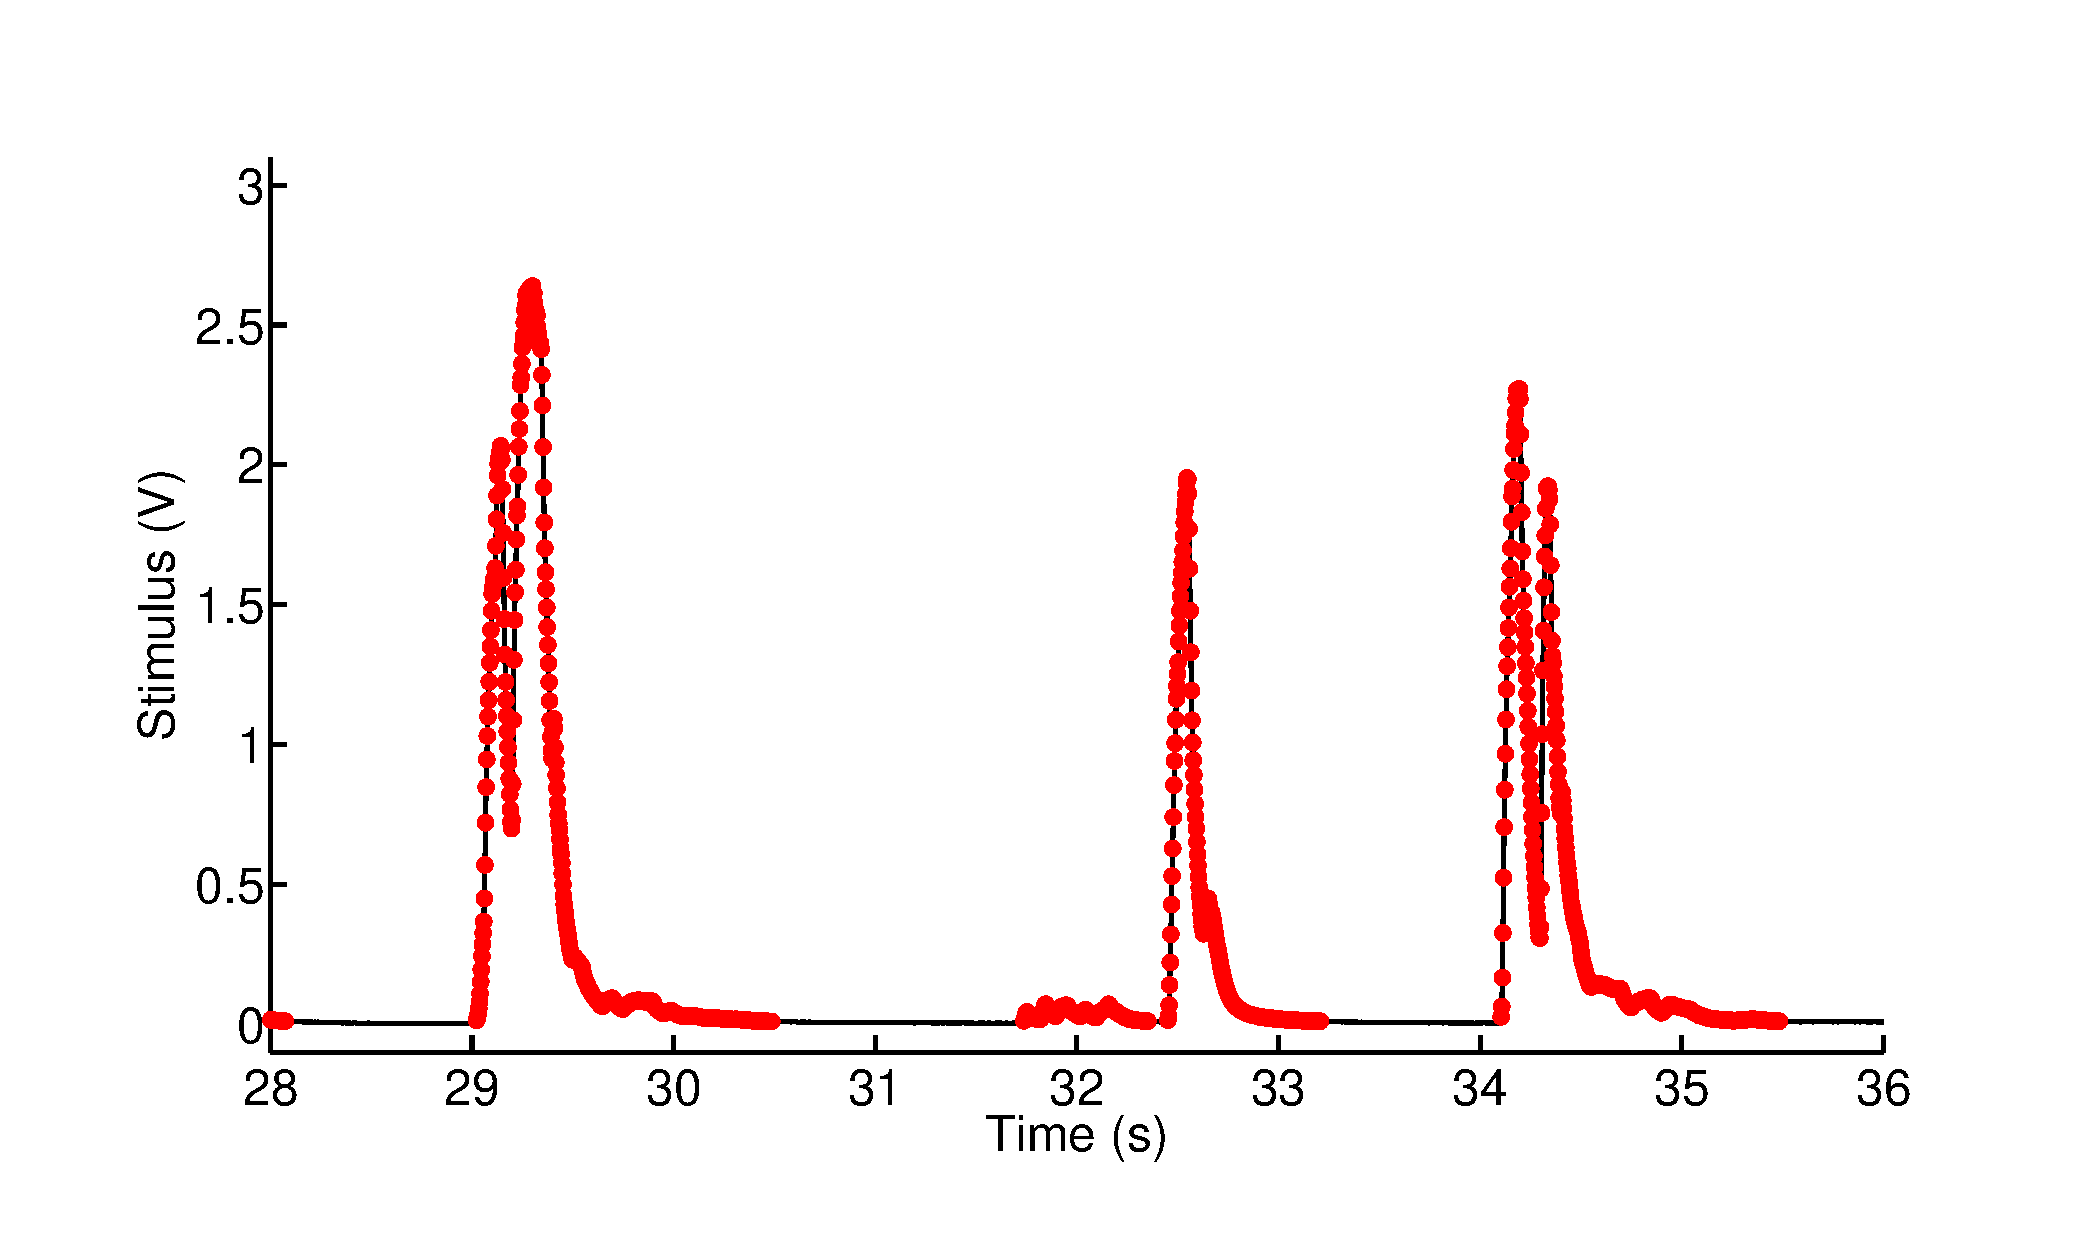
\includegraphics [width=\textwidth]{Mahmut_Data_Analysis_05.pdf}
\begin{par}
The weird shape of the linear filter doesn't bode well for the quality of the linear prediction. The following figure shows the linear fit compared to the data.
\end{par} \vspace{1em}

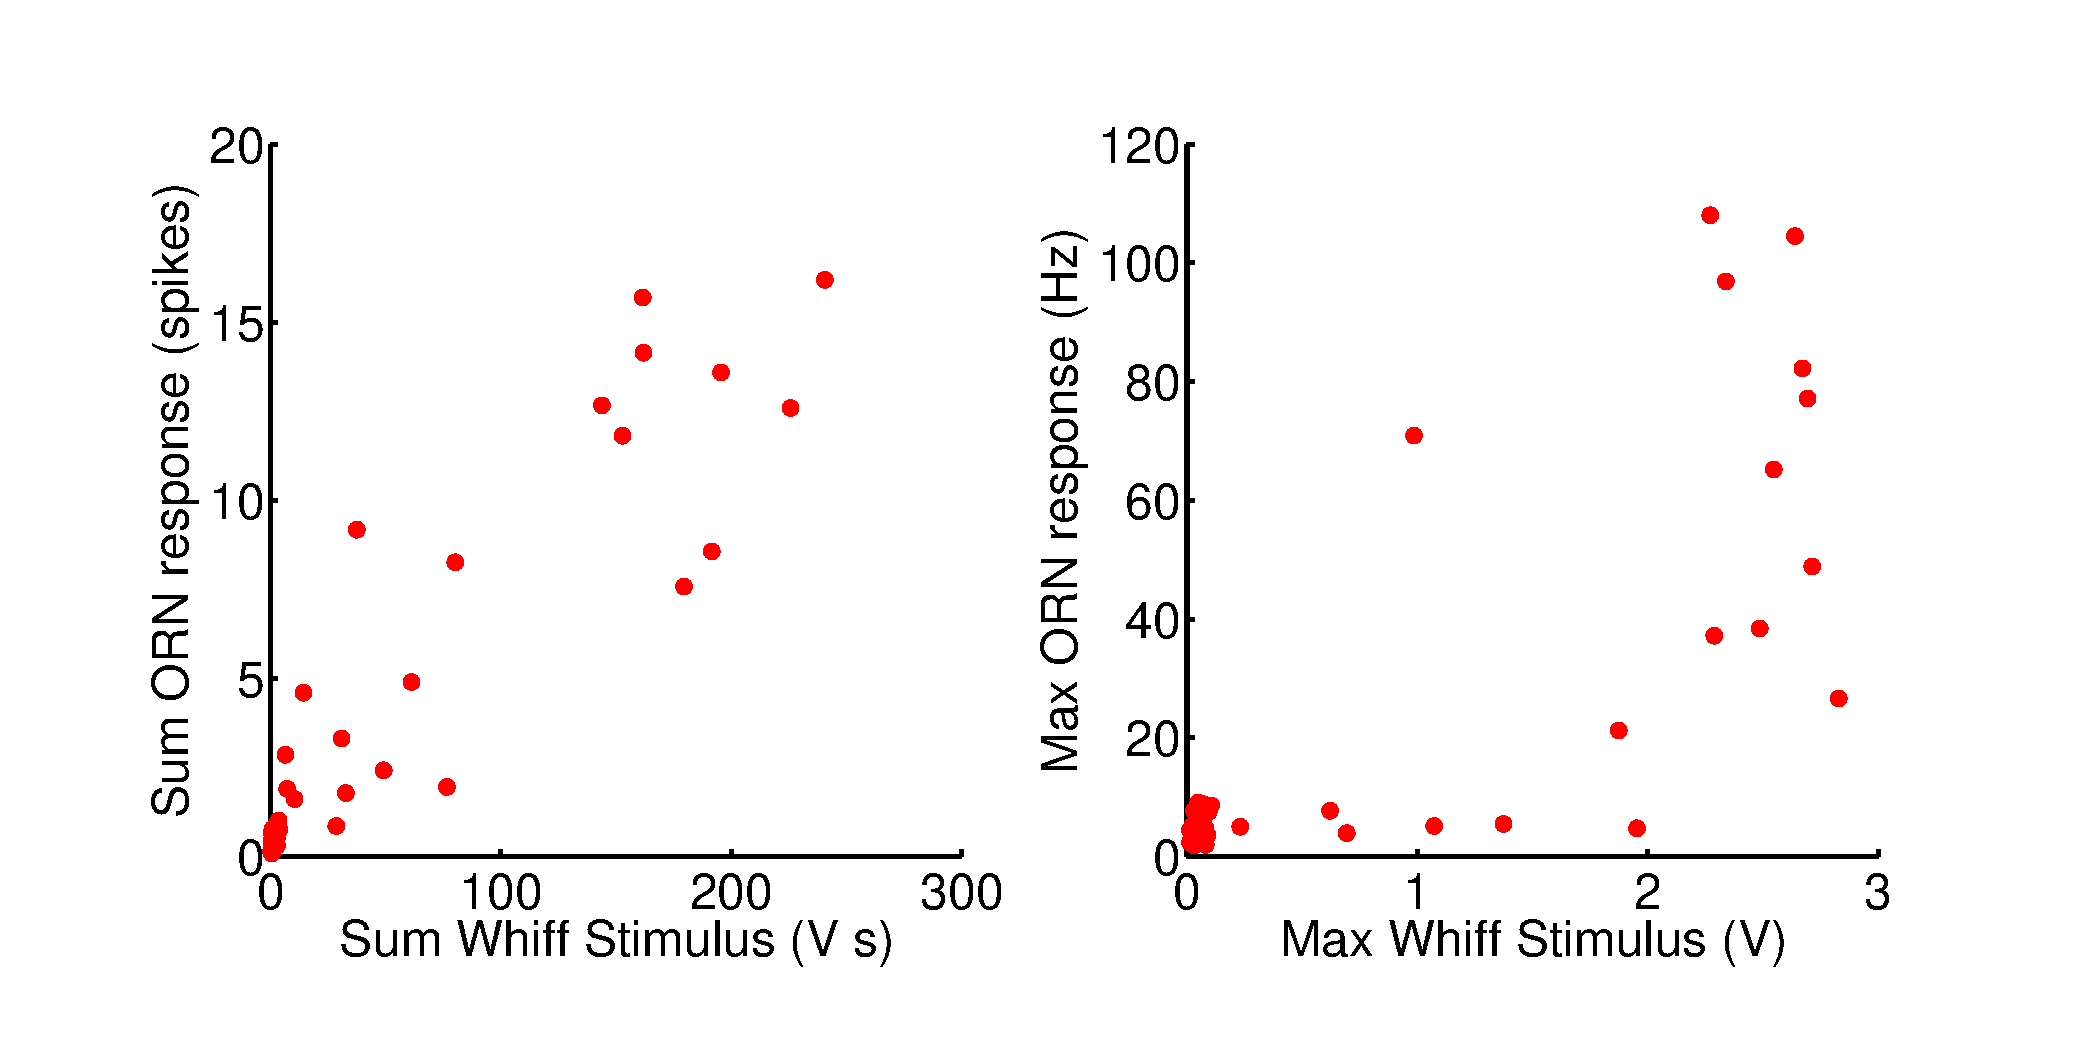
\includegraphics [width=\textwidth]{Mahmut_Data_Analysis_06.pdf}
\begin{par}
The rsquare of the linear fit is:
\end{par} \vspace{1em}

        \color{lightgray} \begin{verbatim}    0.8761

\end{verbatim} \color{black}
    

\subsection*{Gain Analysis: Comparison to Linear Model}

\begin{par}
Even though the linear model does a pretty bad job estimating the response, can we compare the response to the linear model output to see if there is a systematic variation of gain?
\end{par} \vspace{1em}

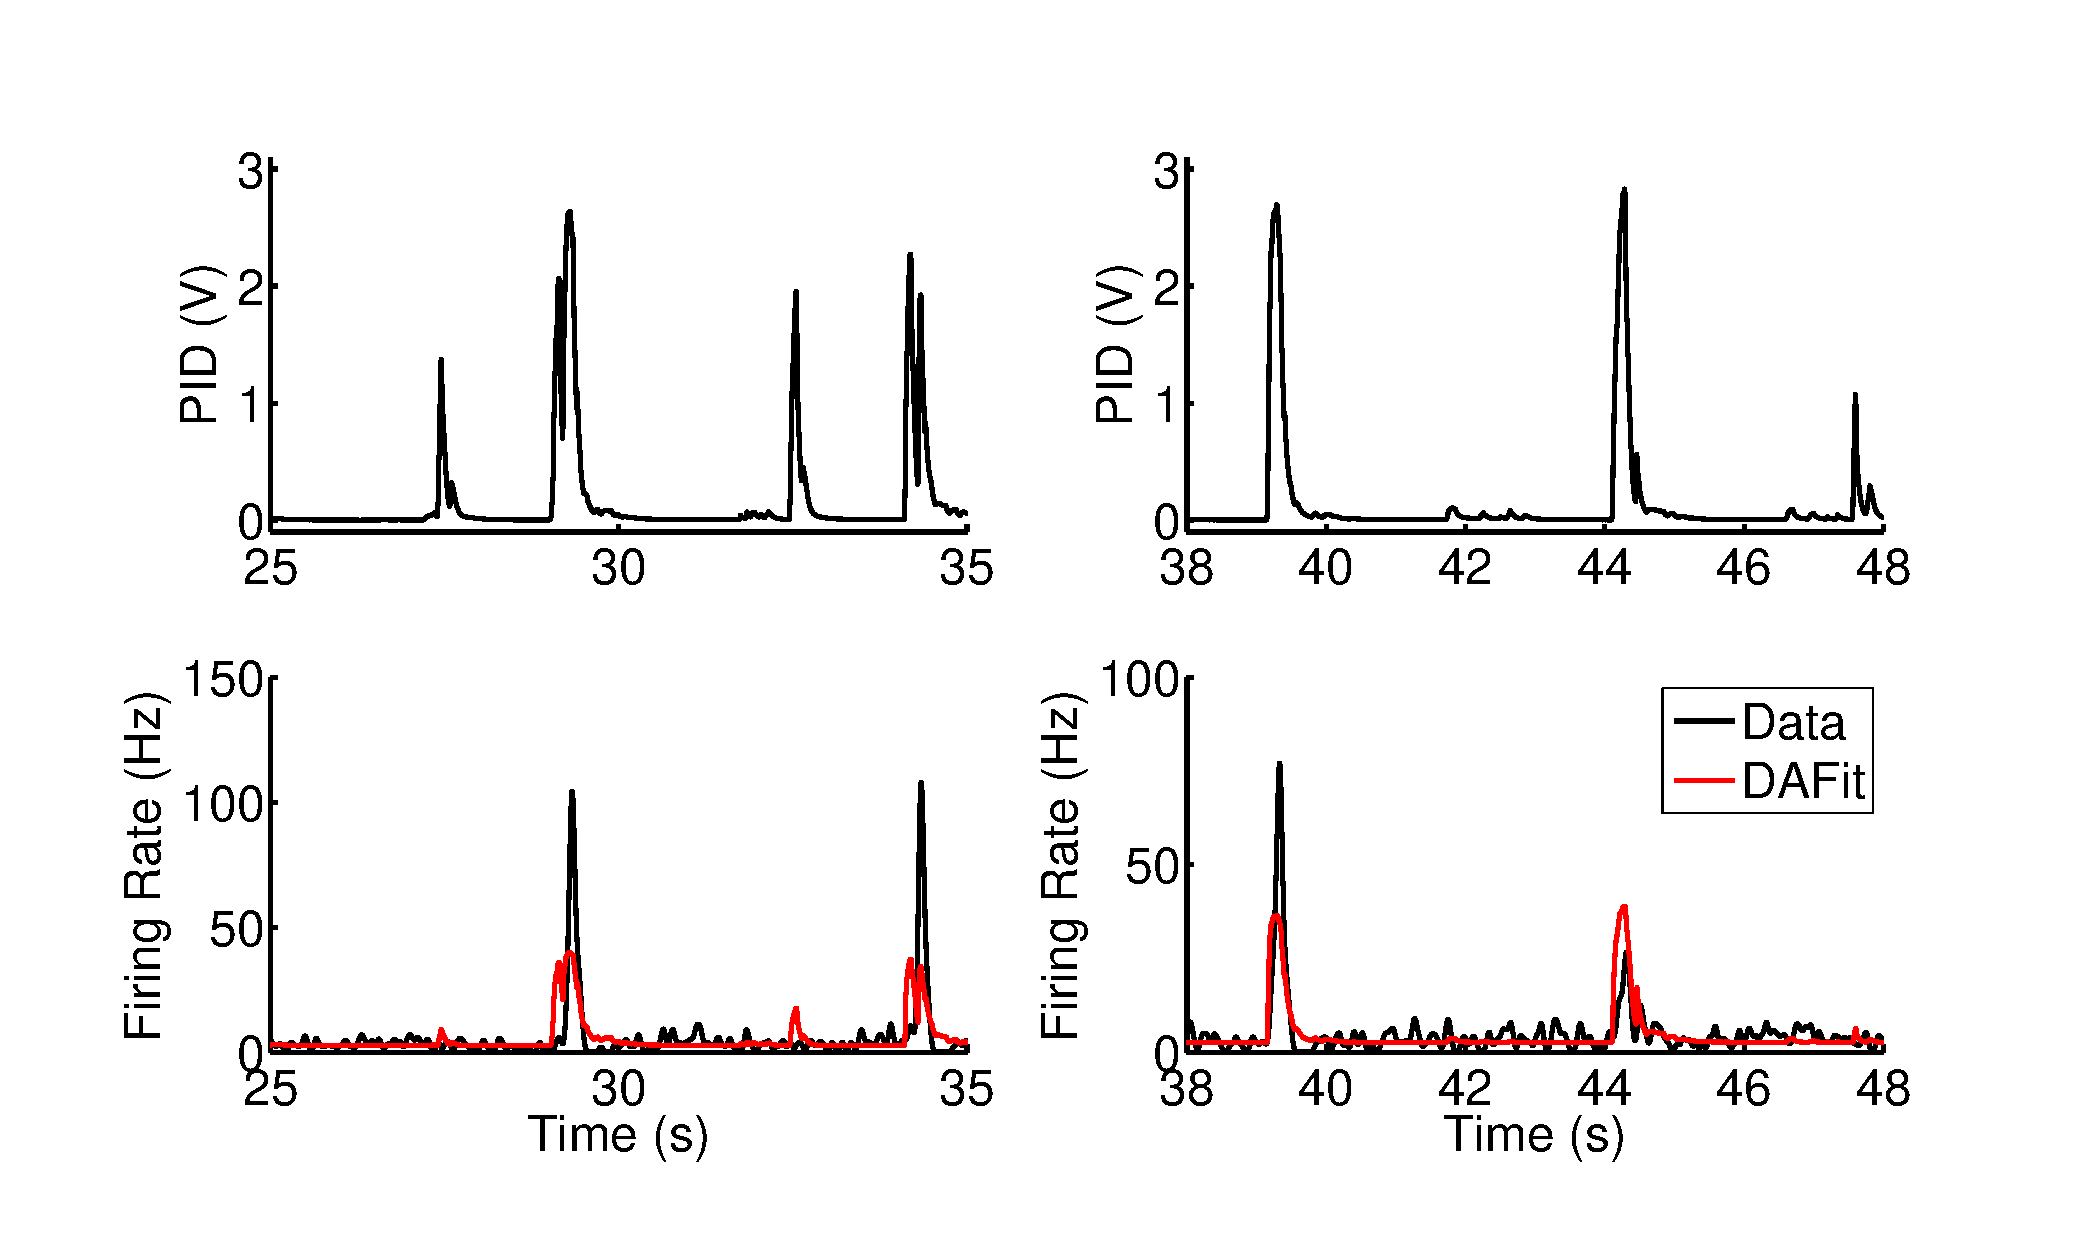
\includegraphics [width=\textwidth]{Mahmut_Data_Analysis_07.pdf}
\begin{par}
Because the fit is so poor, it's hard to fit lines to these clouds of points. We see the general effect where responses to times where the stimulus is low (green) are systematically under-estimated by the linear model, and the responses to times where the stimulus is high (red) are systematically over-estimated by the linear model. However, perhaps this an artefact of the very poor fit?
\end{par} \vspace{1em}
\begin{par}
In the following analysis we redo the gain analysis, but restrict the analysis only to the whiffs.
\end{par} \vspace{1em}

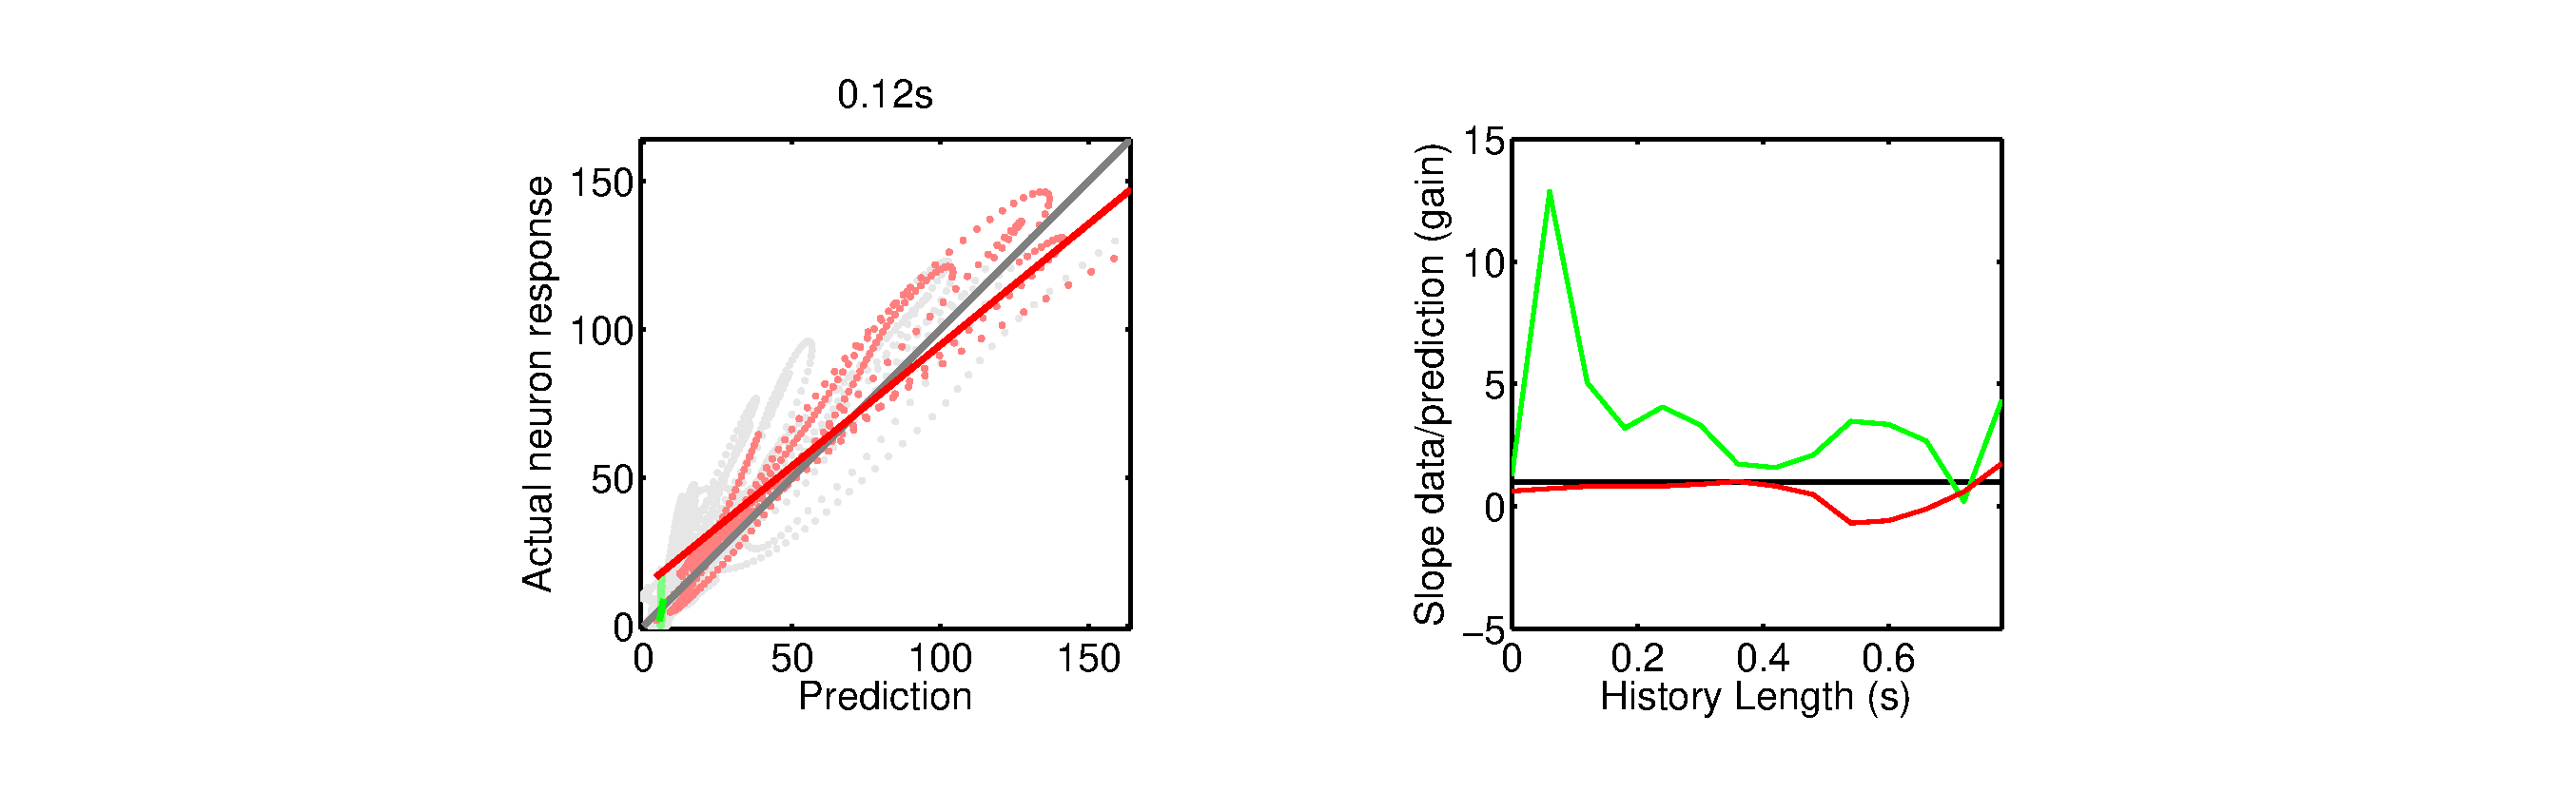
\includegraphics [width=\textwidth]{Mahmut_Data_Analysis_08.pdf}


\subsection*{Fitting a DA Model}

\begin{par}
Can a DA Model explain the responses of this neuron in this dataset? The following figure shows the ORN firing rates and the best-fit DA Model.
\end{par} \vspace{1em}

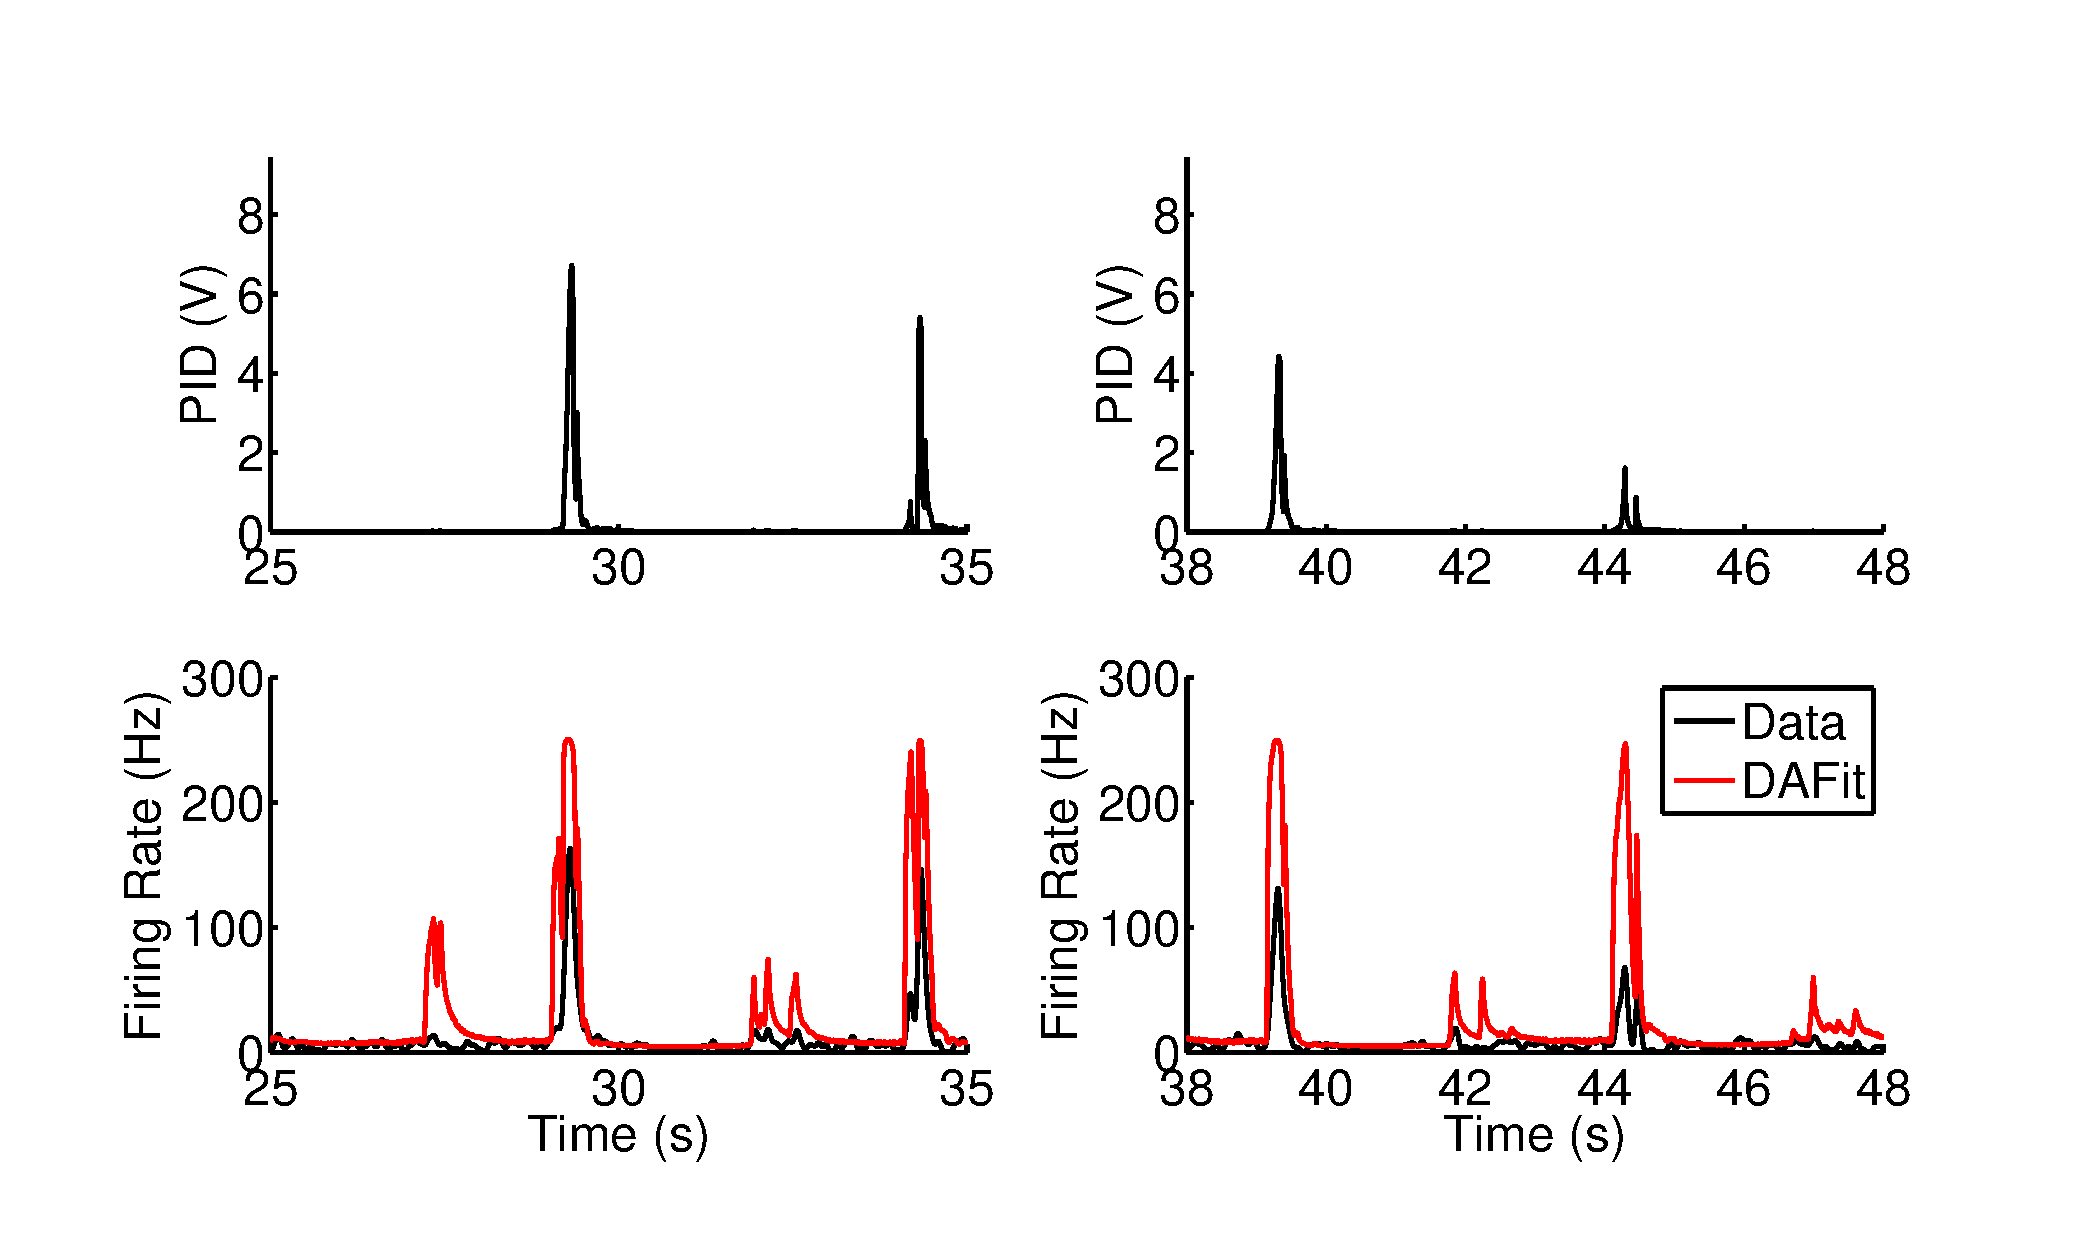
\includegraphics [width=\textwidth]{Mahmut_Data_Analysis_09.pdf}
\begin{par}
The r-square of the DA model fit is:
\end{par} \vspace{1em}

        \color{lightgray} \begin{verbatim}    0.7079

\end{verbatim} \color{black}
    \begin{par}
and the parameters of the model are:
\end{par} \vspace{1em}

        \color{lightgray} \begin{verbatim}        A: 1.6003e+04
        B: 636.9062
        C: 0.1000
    tau_y: 0.9344
      n_y: 2
    tau_z: 92.2188
      n_z: 2
       r0: 4.1985

\end{verbatim} \color{black}
    

\subsection*{Gain Analysis: Comparison to DA Model}

\begin{par}
Does the DA model also show systematic variation of gain for high and low stimuli?
\end{par} \vspace{1em}

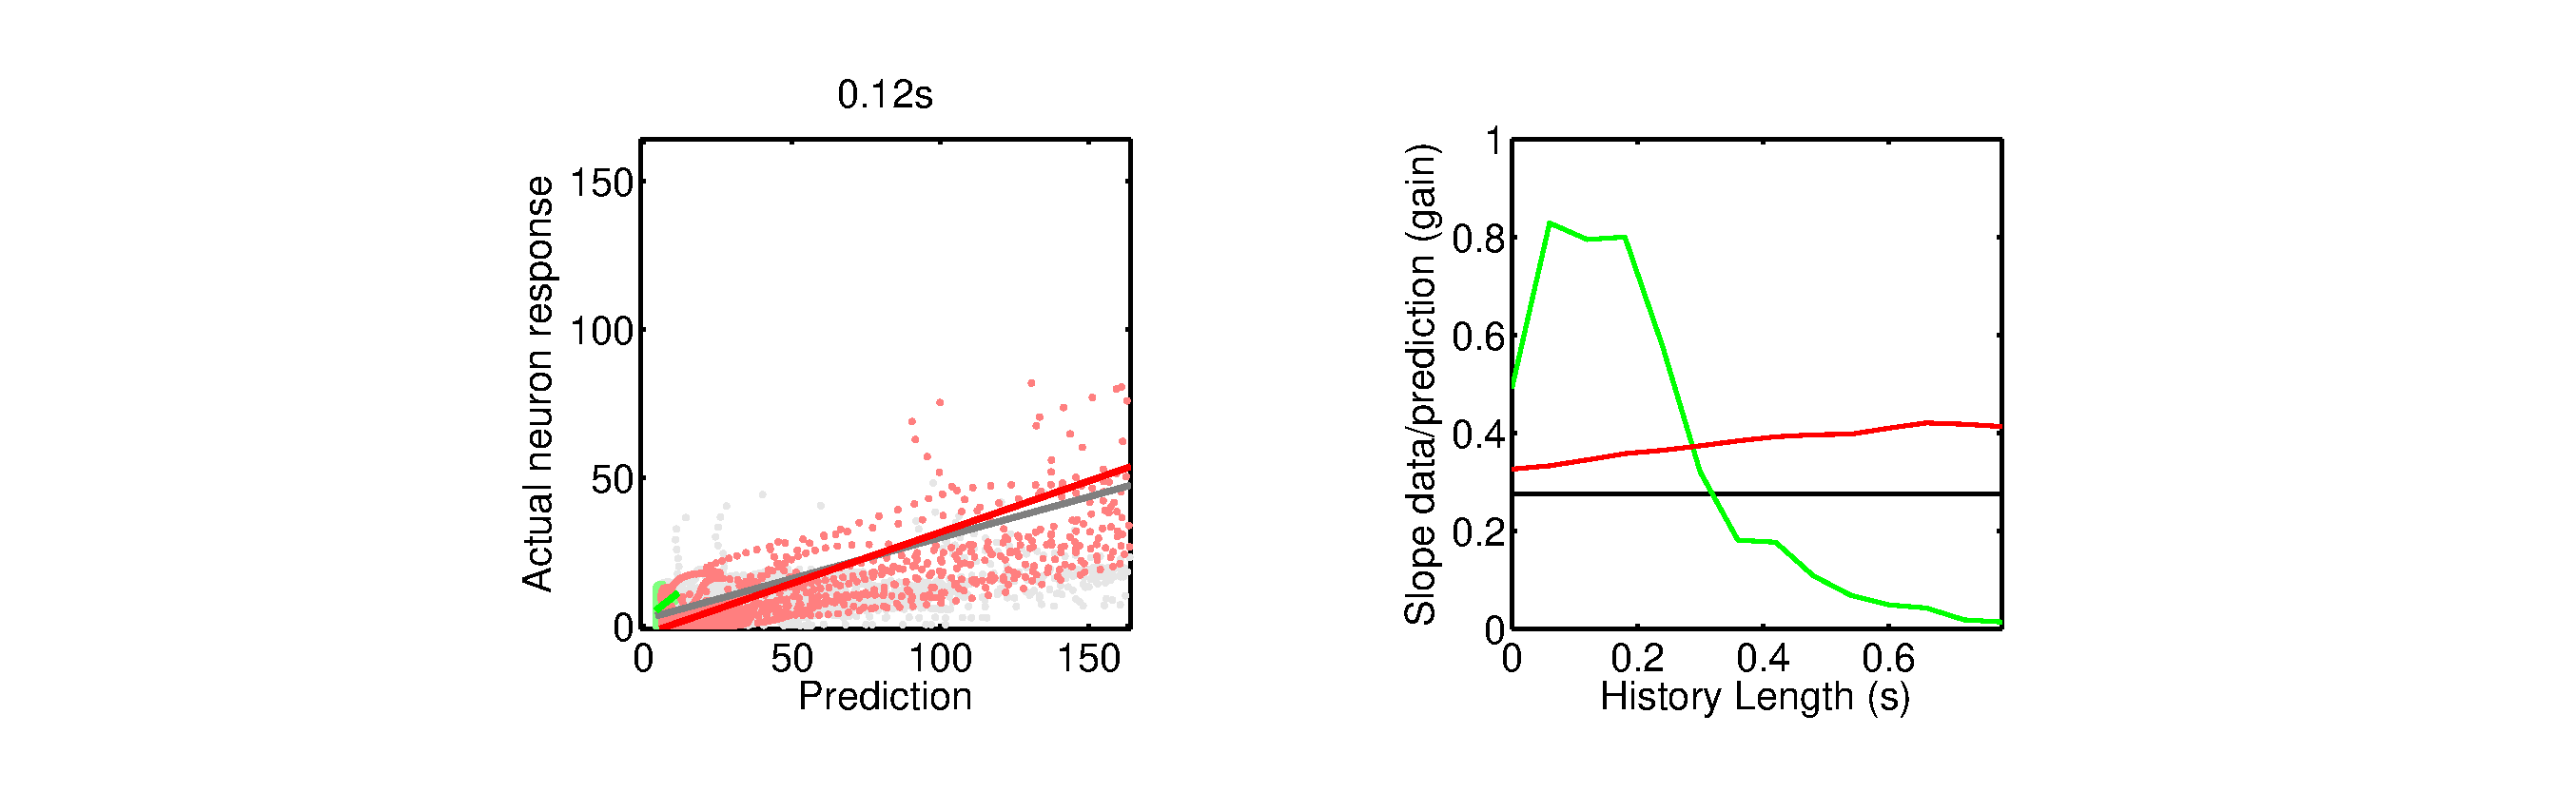
\includegraphics [width=\textwidth]{Mahmut_Data_Analysis_10.pdf}
\begin{par}
Again, we repeat the gain analysis but restrict the analysis only to the whiffs, ignoring the blanks inbetween.
\end{par} \vspace{1em}

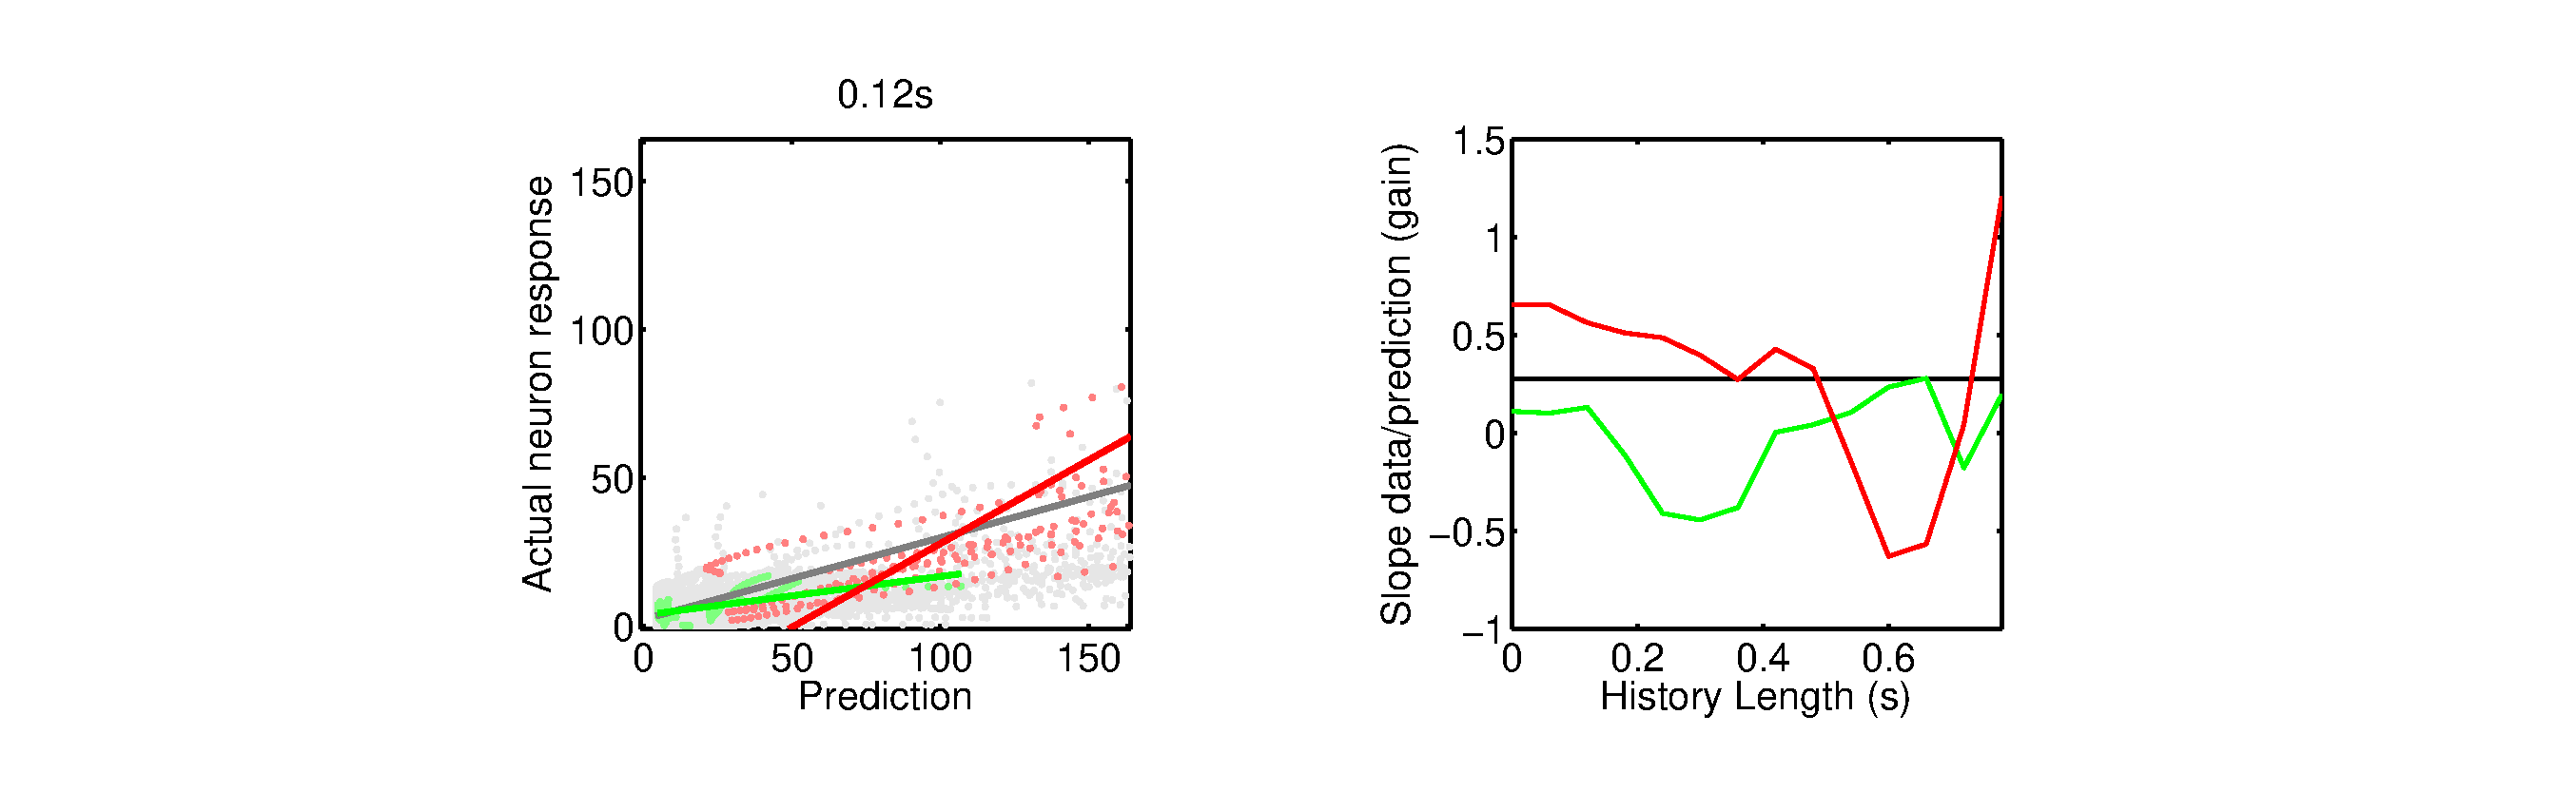
\includegraphics [width=\textwidth]{Mahmut_Data_Analysis_11.pdf}



\end{document}
    
